% This is samplepaper.tex, a sample chapter demonstrating the
% LLNCS macro package for Springer Computer Science proceedings;
% Version 2.20 of 2017/10/04
%
\documentclass[runningheads]{llncs}
%
\usepackage{graphicx}
\usepackage{hyperref}
% Used for displaying a sample figure. If possible, figure files should
% be included in EPS format.
%
% If you use the hyperref package, please uncomment the following line
% to display URLs in blue roman font according to Springer's eBook style:
% \renewcommand\UrlFont{\color{blue}\rmfamily}

\begin{document}
%
\title{Heuristic Search vs Genetic Algorithms: Travelling Salesman Problem}
%
\titlerunning{HS vs GA}
% If the paper title is too long for the running head, you can set
% an abbreviated paper title here
%
\author{Emilio Cortina Labra \orcidID{0000-0002-8191-6023}\\
\email{UO257322@uniovi.es}}
%
\authorrunning{E. Cortina Labra}
% First names are abbreviated in the running head.
% If there are more than two authors, 'et al.' is used.
%
\institute{Sistemas Inteligentes. Grado en Ingeniería Informática.\\
 EII. Universidad de Oviedo. Campus de los Catalanes. E-33007. Oviedo\\
}
%
\maketitle              % typeset the header of the contribution
%
\begin{abstract}
The abstract should briefly summarize the contents of the paper in
150--250 words.

\keywords{TSP  \and A* \and Genetic Algorithms \and heuristics.}
\end{abstract}
%
%
%
\section{Introduction}
Please note that the first paragraph of a section or subsection is
not indented. The first paragraph that follows a table, figure,
equation etc. does not need an indent, either.

Subsequent paragraphs, however, are indented.

%
%
%
\section{Travel Salesman Problem (TSP)}
\subsection{History}
"In 1832, a German travelling salesman published a handbook describing his profession. His name is unknown; he only stated that the book was written by “one old travelling salesman.” However, he has come down in history thanks to a rather simple and quite obvious observation. He pointed out that when one goes on a business trip, one should plan it carefully; by doing so, one can “win” a great deal of time and increase the trip’s “economy.” Two centuries later, mathematicians and scientists are still struggling with what is now known as the “Travelling Salesman Problem” (TSP)"~\cite{ref_article_bridgew}

\subsection{Description}
The problem defines a set of cities along with the associated cost of travel between each pair of them. The goal of the problem is to find the cheapest path or circuit that goes through every single city exactly once, and finally returns to the starting position.

Given the simplicity of the statement of this problem, it may seem like an easy task to solve. It's only about thinking on the different possible paths, add the costs of each one and then compare the outcomes to find out which was the one with the least total cost. This is feasible to compute even for a human when we are dealing with small instances of the problem, but it is not trivial at all to compute for bigger instances of the problem, even for powerful computers.

As it can be seen in Table~\ref{tab1} the number of the different possibilities grows rapidly with the number of cities defined in the instance of the problem.

\begin{table}
\caption{Number of possibilities for each instance size of the problem.}\label{tab1}
\begin{tabular}{ |p{0.3\linewidth}|p{0.7\linewidth}| }
\hline
Number of cities &  Number of possibilities \\
\hline
5 &  5! = 5*4*3*2*1 = 120\\
25 & 25! = 25*24*23*...*3*2*1 = 15,511,210,043,330,985,984, 000,000 \\
100 & 100!  = 93,326,215,443,944,152,681,699,238,856,266,700, 490,715,968,264,381,621,468,592,963,895,217,599, 993,229,915,608,941,463,976,156,518,286,253,697, 920,827,223,758,251,185,210,916,864,000,000,000, 000,000,000,000,000 \\
\hline
\end{tabular}
\end{table}

\subsection{Applications}
Many different fields make use of the TSP to solve several problems. Some of these use cases are obvious, like the planning of school bus routes or the routing of a laundry van, but others can seem more far-fetched at first.
A few applications of the problem will be discussed in this section.

\subsubsection{Logistics}
This is the category that the TSP was originally described for. Different transport industries are using systems that calculate routes by means of the TSP. Although it was Merill Flood ~\cite{ref_book_flood} who first introduced the idea of applying the problem to plan school bus routes back in 1956, this application is still in use nowadays, with several companies building software solutions for it.

\subsubsection{Genome sequencing}
By making analogies of the problem, researchers working on genome sequencing at the National Institute of Health have used the TSP to construct radiation hybrid maps. They integrated local maps into a single radiation hybrid map for a genome, the cities being the local maps and the cost of travel being a measure of how likely one local map will immediately follow another ~\cite{ref_article_genome}.

\subsubsection{Telescopes}
The problem can also be used with locations that cannot be physically reached or visited, for example with planets, stars and galaxies.
For observing these objects telescopes must be set into position. The process of rotating the equipment is called {\itshape slewing}, and 
for bigger telescopes it is a complicated and time-consuming movement that has to be performed by computer-driven motors.
By making use of the TSP the aim is to minimize this slewing movement for a given set of celestial objects. In the TSP these objects 
would represent every city, and the costs is the slewing time to move the telescope from one object to the next ~\cite{ref_book_tsp}.


%
%
%
\section{Heuristic search algorithms}
Heuristic search algorithms are a special kind of State-space search algorithms. Contrary to uninformed state-space search
algorithms, Heuristic algorithms make use of knowledge about the problem they are trying to solve in order to lead the search
towards more promising areas of the search space, so that fewer nodes are expanded to find the solution.

However, the use of knowledge about the problem comes with a trade-off, which is the computational cost of taking into account this information.

\subsection{A* algorithm}
This is algorithm is the most popular choice for pathfinding, as it's flexible and can be used in a wide range 
of domains ~\cite{ref_url_a_stanford}.
A* algorithm is a special case of the Best-first search algorithm ~\cite{ref_url_bfs_washington,ref_url_bfs_wiki}, 
that defines the {\itshape evaluation function} in a particular way, given any node {\itshape n}
 from the search space:
 \begin{definition}
g*(n) is the cost of the shortest path from the starting position to n.
\end{definition}
 \begin{definition}
h*(n) is the cost of the shortest path from the starting n to the nearest objective.
\end{definition}
\begin{definition}
f*(n) = g*(n) + h*(n) is the cost of the shortest path from the starting position to an objective passing through n.
\end{definition}
\begin{definition}
C* = f*(initial) = h*(initial) is the cost of the optimal solution.
\end{definition}

But these are ideal values that cannot be exactly calculated for big problems in a reasonable amount of time.
If we knew these values for every node, we would have a fast algorithm that only expands states that lead to the optimal solution.

However, we can work with approximations of the functions above.
 \begin{definition}
g(n) is the cost of the shortest path from the starting position to n, found so far.  
\end{definition}
 \begin{definition}
h(n) is the heuristic function.
\end{definition}
\begin{definition}
f(n) = g(n) + h(n) is the evaluation function we will use.
\end{definition}

\subsubsection{Heuristic function}
The heuristic function {\itshape h(n)} is an approximation of {\itshape h*(n)}. Designing the heuristic
requires some knowledge about the domain that is usually obtained by analyzing the problem.
This function deeply determines the behaviour and properties of the A* algorithms, such as its admisibility, monotony,
consistency... ~\cite{ref_url_heuristic_stanford}.\\
For example, using a more informed heuristic, that is, one with a value is closer to that of {\itshape h*(n)} will result on A*
expanding fewer nodes at the cost of computational overhead.
On the contrary, using a less informed heuristic results on less computational overhead at the cost of expanding more nodes
to find the optimal solution. It can also be the case in which an optimal solution is not found if the heuristic is not admisible, that  is {\itshape h(n)\textgreater h*(n)}.

\subsection{Static-weighted A* algorithm}
It is usually assumed that increasing the weight on the heuristic will decrease search time, and that greedy search will provide the fastest search.
Although there is no formal guarantee for this, weighted A* relies on this mechanism to speed up the searching process, and is the most popular
satisficing algorithm for heuristic search ~\cite{ref_article_a_weighted}.

For achieving this, static-weighted A* defines the following evaluation function:

 \begin{equation}
f(n) = g(n) + \varepsilon * h(n)
\end{equation}

where

\begin{equation}
\varepsilon > 1
\end{equation}

Static-weighted A* has a bias towards states that are closer to the goal ~\cite{ref_url_a_carneige}.
%
%
%
\section{Genetic algorithms}
Genetic algorithms are search and optimization algorithms based on the mechanisms of natural evolution. By mimicking this process,
they are able to "evolve" solutions to real world problems if they have been suitably encoded ~\cite{ref_url_a_carneige}. 

%
%
%
\section{Solving the Travel Salesman Problem}
Esta sección debe tener varias subsecciones en las que se describan los algoritmos de búsqueda utilizados.

\subsection{Problem solving using heuristic search}
Please note that the first paragraph of a section or subsection is
not indented. The first paragraph that follows a table, figure,
equation etc. does not need an indent, either.

\subsection{Problem solving using genetic algorithms}
Please note that the first paragraph of a section or subsection is
not indented. The first paragraph that follows a table, figure,
equation etc. does not need an indent, either.

%
%
%
\section{Experimental results}
Esta sección debe tener varias subsecciones en las que se describan los algoritmos de búsqueda utilizados.



\noindent Displayed equations are centered and set on a separate
line.
\begin{equation}
x + y = z
\end{equation}
Please try to avoid rasterized images for line-art diagrams and
schemas. Whenever possible, use vector graphics instead (see
Fig.~\ref{fig1}).

\begin{figure}
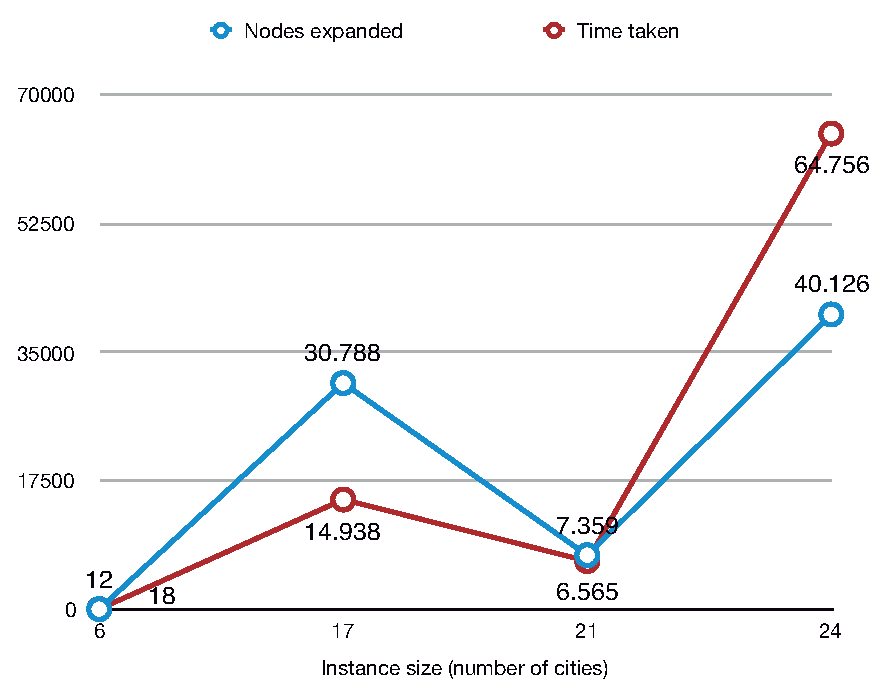
\includegraphics[width=\textwidth]{prueba.eps}
\caption{A figure caption is always placed below the illustration.
Please note that short captions are centered, while long ones are
justified by the macro package automatically.} \label{fig1}
\end{figure}

\begin{theorem}
This is a sample theorem. The run-in heading is set in bold, while
the following text appears in italics. Definitions, lemmas,
propositions, and corollaries are styled the same way.
\end{theorem}
%
% the environments 'definition', 'lemma', 'proposition', 'corollary',
% 'remark', and 'example' are defined in the LLNCS documentclass as well.
%
\begin{proof}
Proofs, examples, and remarks have the initial word in italics,
while the following text appears in normal font.
\end{proof}

%
% ---- Bibliography ----
%
% BibTeX users should specify bibliography style 'splncs04'.
% References will then be sorted and formatted in the correct style.
%
% \bibliographystyle{splncs04}
% \bibliography{mybibliography}
%
\begin{thebibliography}{8}

\bibitem{ref_article_bridgew}
Pacha-Sucharzewski, Mateusz (2011). Analysis of the “Travelling Salesman Problem” and an Application of Heuristic Techniques for Finding a New Solution. Undergraduate Review, 7, 81-86.
Available at \url{http://vc.bridgew.edu/undergrad_rev/vol7/iss1/17}

\bibitem{ref_article_belal}
Belal Ahmed et al 2017 IOP Conf. Ser.: Mater. Sci. Eng. 263 042085

\bibitem{ref_book_tsp}
David L. Applegate (2011). The traveling salesman problem: a computational study.
Princeton University Press, Year: 2006

\bibitem{ref_book_flood}
Flood, M. M. 1956. The traveling-salesman problem. Operations Research 4, 61–75.

\bibitem{ref_article_genome}
R. Agarwala, D.L. Applegate, D. Maglott, G.D. Schuler, and A.A. Schaffler. A Fast and Scalable Radiation Hybrid Map Construction and Integration Strategy.
\url{https://www.ncbi.nlm.nih.gov/genome/rhmap/manuscript.ps}

\bibitem{ref_url_a_stanford}
Amit’s Thoughts on Pathfinding - Introduction to A*.\\
\url{http://theory.stanford.edu/~amitp/GameProgramming/AStarComparison.html}\\
Last accessed October 23rd 2019.

\bibitem{ref_url_a_carneige}
Maxim Likhachev. A* and Weighted A* Search.\\
Carnegie Mellon University.\\
\url{https://www.cs.cmu.edu/~motionplanning/lecture/Asearch_v8.pdf}\\
Last accessed October 23rd 2019.

\bibitem{ref_url_bfs_washington}
Best-first search. CSE 326: Data Structures, Summer 2003.\\
University of Washington Computer Science and Engineering\\
\url{https://courses.cs.washington.edu/courses/cse326/03su/homework/hw3/bestfirstsearch.html}
Last accessed October 23rd 2019.

\bibitem{ref_url_bfs_wiki}
Best-first search. Wikipedia.\\
\url{https://en.wikipedia.org/wiki/Best-first_search}
Last accessed October 23rd 2019.

\bibitem{ref_url_heuristic_stanford}
Amit’s Thoughts on Pathfinding - Heuristics.\\
\url{http://theory.stanford.edu/~amitp/GameProgramming/Heuristics.html}\\
Last accessed October 23rd 2019.

\bibitem{ref_article_a_weighted}
Christopher Wilt and Wheeler Ruml. When does Weighted A* Fail?\\
University of New Hampshire\\
\url{http://www.cs.unh.edu/~ruml/papers/wted-astar-socs-12.pdf}



\end{thebibliography}
\end{document}
